% Math Packages
\usepackage{amsmath, amsfonts, mathtools, amsthm,extarrows, amssymb,bbm}

\usepackage{esint}

% Programming Packages
\usepackage{pythonhighlight}

% Color -> #D65B53
\definecolor{CustomColorChoice}{cmyk}{0, 0.99, 0.87, 0.18, 0}

% Citations
\usepackage{natbib}

\usepackage{hyperref}
\newcommand{\link}[2]{{\bfseries\color{CustomColorChoice!85}\href{#1}{#2}}}
 
% Figures
\usepackage{graphicx}
\graphicspath{{./figures/}}
\usepackage{float}
\usepackage{caption}
\usepackage{subcaption}

% Congruent Modulo
\newcommand{\cmod}[3]{ #1 \text{ } \equiv \text{ } #2 \text{ } (\mathrm{mod} \ #3)}

% Contents
\usepackage{tocloft}

\renewcommand\contentsname{Summary of Contents}
\renewcommand\cfttoctitlefont{\Large\bfseries\sffamily}
\renewcommand\cftaftertoctitle{\hfill}

% Formatting
\usepackage[utf8]{inputenc}
\usepackage[T1]{fontenc}

% Tables
\usepackage{booktabs, tabularx}

% Shortcuts (N, R, Z, etc.)
\newcommand\N{\ensuremath{\mathbb{N}}}
\newcommand\Prob{\ensuremath{\mathbb{P}}}
\newcommand\R{\ensuremath{\mathbb{R}}}
\newcommand\Z{\ensuremath{\mathbb{Z}}}
\renewcommand\O{\ensuremath{\emptyset}}
\newcommand\Q{\ensuremath{\mathbb{Q}}}
\newcommand\C{\ensuremath{\mathbb{C}}}
\newcommand\fpa{\tilde{f}_{\texttt{FP}}}
\newcommand\ipa{\tilde{f}_{\texttt{IP}}}
\newcommand\deriv{\frac{d f}{d x}}

% Floor and Cieling
\newcommand{\floor}[1]{\left\lfloor #1 \right\rfloor}
\newcommand{\ceil}[1]{\left\lceil #1 \right\rceil}
\newcommand{\Hess}{$\mathbf{H}(f)$}
% Title Formatting
\titleformat*{\section}{\Large\bfseries\sffamily}
\titleformat*{\subsection}{\large\bfseries\sffamily}
\titleformat*{\subsubsection}{\itshape\sffamily}

% Horizontal Line
\newcommand{\LineBreak}{\vspace{0.5pc} \noindent \textcolor{CustomColorChoice}{\makebox[\linewidth]{\rule{\linewidth}{0.4pt}}} \vspace{0.5pc}}

\newcommand{\NewLine}{\[ \]}

% Example Box Formatting
\usepackage[most]{tcolorbox}

\tcbuselibrary{theorems}
\newtcbtheorem[]{ex}{\textbf{Example}}{
  	breakable,
    colback=CustomColorChoice!5,
    colframe=CustomColorChoice!85,
    fonttitle=\sffamily\color{White}
  }{def}

 % Theorem and Proof Formatting
\usepackage{thmtools}

\declaretheoremstyle[
    headfont=\bfseries\sffamily\color{CustomColorChoice!85},
    bodyfont=\normalfont,
    mdframed={
        linewidth=2pt,
        usetwoside=false,
        rightline=false, topline=false, bottomline=false,
        linecolor=CustomColorChoice!85, backgroundcolor=CustomColorChoice!5,
    }
]{defnbox}

\declaretheoremstyle[
    headfont=\bfseries\sffamily\color{Black},
    bodyfont=\normalfont,
    mdframed={
        linewidth=2pt,
        rightline=false, topline=false, bottomline=false,
        linecolor=CustomColorChoice!85, backgroundcolor=white,
    }
]{thmbox}


\declaretheoremstyle[
    headfont=\bfseries\sffamily\color{Black},
    bodyfont=\normalfont,
    mdframed={
        linewidth=2pt,
        rightline=false, topline=false, bottomline=false,
        linecolor=CustomColorChoice!15, backgroundcolor=white,
    }
]{marginbox}

\declaretheoremstyle[
    headfont=\bfseries\sffamily\color{Black},
    bodyfont=\normalfont,
    mdframed={
        linewidth=2pt,
        rightline=false, topline=false, bottomline=false,
        linecolor=CustomColorChoice!85, backgroundcolor=white,
    }
]{rmkbox}

\declaretheoremstyle[
    headfont=\bfseries\sffamily\color{Black},
    bodyfont=\normalfont,
    numbered=no,
    mdframed={
        linewidth=2pt,
        rightline=false, topline=false, bottomline=false,
        linecolor=white, backgroundcolor=white,
    }
]{corbox}

\declaretheoremstyle[
    headfont=\bfseries\sffamily\color{CustomColorChoice!85},
    bodyfont=\normalfont,
    numbered=no,
    mdframed={
        linewidth=2pt,
        rightline=false, topline=false, bottomline=false,
        linecolor=white, backgroundcolor=white,
    },
    qed=\qedsymbol
]{proofbox}

 \declaretheorem[style=thmbox, numbered=yes, name=Lemma]{lem}
 \declaretheorem[style=thmbox, numbered=yes, name=Theorem]{thm}
  \declaretheorem[style=thmbox, numbered=yes, name=Proposition]{prop}
  \declaretheorem[style=thmbox, numbered=no, name=Conjecture]{conj}
 \declaretheorem[style=rmkbox, numbered=no, name=Note]{note}
 \declaretheorem[style=rmkbox, numbered=no, name=Remark]{rmk}
 \declaretheorem[style=corbox, numbered=no, name=Corollary]{cor}
  \declaretheorem[style=corbox, numbered=no, name=Overview]{oproof}
 \declaretheorem[style=defnbox, numbered=no, name=Definition]{defn}
 \declaretheorem[style=proofbox, numbered=no, name=Proof]{replacementproof}

 \renewenvironment{proof}[1][\proofname]{\vspace{-10pt}\begin{replacementproof}}{\end{replacementproof}}

% Title Page

\makeatletter
\renewcommand{\maketitlepage}{
    \cleardoublepage{
        \begin{fullwidth}
        
        \fontsize{10}{14}\selectfont\par\noindent{\textbf{Semester}: Fall 2022}
        \fontsize{10}{14}\selectfont\par\noindent{\textbf{Instructor}: Kamran, Niky}

        \vspace{2pc}
        
        \fontsize{36}{40}\selectfont\par\noindent{Honours Vector Calculus}
        
        \begin{center}
        
        \vfill
        
        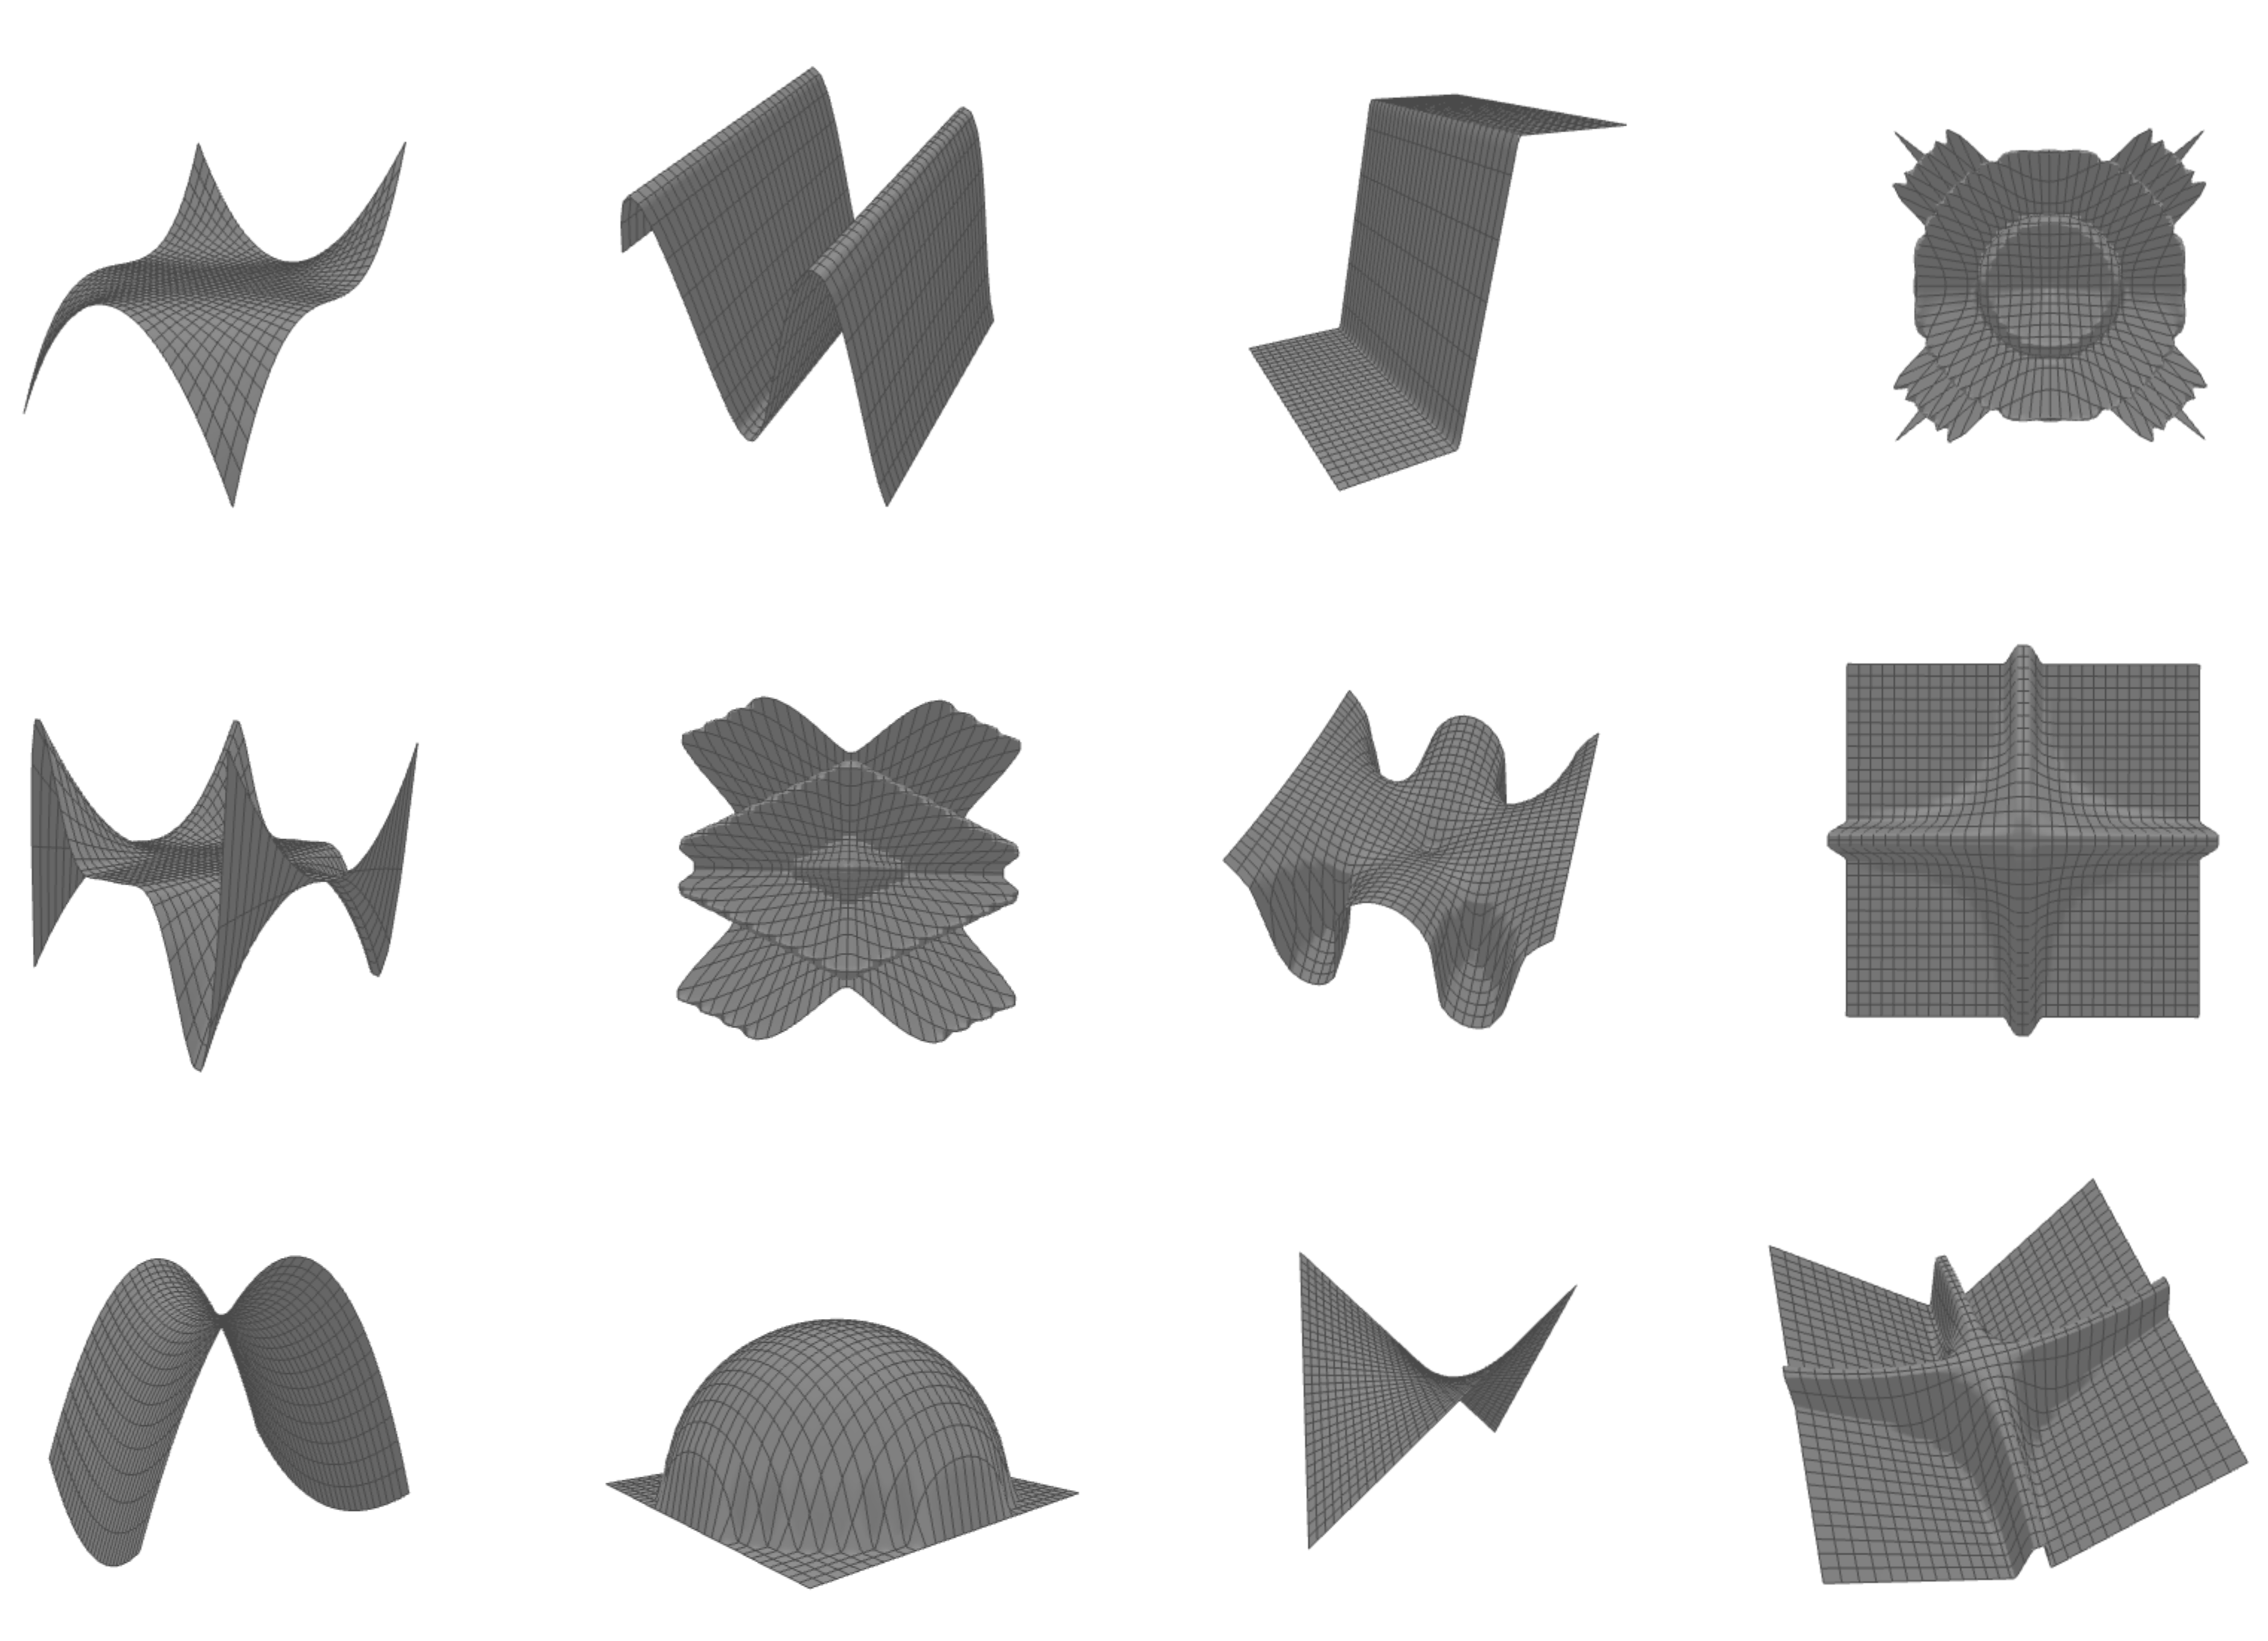
\includegraphics[width=\linewidth]{figures/title/fig-3.png}
        \end{center}
        
        \vfill
        
        \fontsize{10}{14}\selectfont\par\noindent\thanklesspublisher{\textbf{Course Content.}  Partial derivatives and differentiation of functions in several variables; Jacobians; maxima and minima; implicit functions. Scalar and vector fields; orthogonal curvilinear coordinates. Multiple integrals; arc length, volume and surface area. Line and surface integrals; irrotational and solenoidal fields; Green's theorem; the divergence theorem. Stokes' theorem; and applications.}
        \end{fullwidth}
    }
    \thispagestyle{empty}
    \clearpage
}
\makeatother